\documentclass{beamer}
\mode<presentation>
\usepackage{amsmath}
\usepackage{amssymb}
%\usepackage{advdate}
\usepackage{adjustbox}
\usepackage{subcaption}
\usepackage{enumitem}
\usepackage{multicol}
\usepackage{mathtools}
\usepackage{listings}
\usepackage{url}
\def\UrlBreaks{\do\/\do-}
\usetheme{Boadilla}
\usecolortheme{lily}
\setbeamertemplate{footline}{
  \leavevmode%
  \hbox{%
    \begin{beamercolorbox}[wd=.9\paperwidth,ht=2.25ex,dp=1ex,left]{author in head/foot}%
      \hspace{1em} Balaji B % Your name here
    \end{beamercolorbox}%
    \begin{beamercolorbox}[wd=.1\paperwidth,ht=2.25ex,dp=1ex,right]{author in head/foot}%
      \insertframenumber{} / \inserttotalframenumber\hspace*{2ex}
    \end{beamercolorbox}}%
}
\setbeamertemplate{navigation symbols}{}

\providecommand{\nCr}[2]{\,^{#1}C_{#2}} % nCr
\providecommand{\nPr}[2]{\,^{#1}P_{#2}} % nPr
\providecommand{\mbf}{\mathbf}
\providecommand{\pr}[1]{\ensuremath{\Pr\left(#1\right)}}
\providecommand{\qfunc}[1]{\ensuremath{Q\left(#1\right)}}
\providecommand{\sbrak}[1]{\ensuremath{{}\left[#1\right]}}
\providecommand{\lsbrak}[1]{\ensuremath{{}\left[#1\right.}}
\providecommand{\rsbrak}[1]{\ensuremath{{}\left.#1\right]}}
\providecommand{\brak}[1]{\ensuremath{\left(#1\right)}}
\providecommand{\lbrak}[1]{\ensuremath{\left(#1\right.}}
\providecommand{\rbrak}[1]{\ensuremath{\left.#1\right)}}
\providecommand{\cbrak}[1]{\ensuremath{\left\{#1\right\}}}
\providecommand{\lcbrak}[1]{\ensuremath{\left\{#1\right.}}
\providecommand{\rcbrak}[1]{\ensuremath{\left.#1\right\}}}
\theoremstyle{remark}
\newtheorem{rem}{Remark}
\newcommand{\sgn}{\mathop{\mathrm{sgn}}}
\providecommand{\abs}[1]{$\left \vert#1\right\vert$}
\providecommand{\res}[1]{\Res\displaylimits_{#1}} 
\providecommand{\norm}[1]{\lVert#1\rVert}
\providecommand{\mtx}[1]{\mathbf{#1}}
\providecommand{\mean}[1]{E$\left[ #1 \right ]$}
\providecommand{\fourier}{\overset{\mathcal{F}}{ \rightleftharpoons}}
%\providecommand{\hilbert}{\overset{\mathcal{H}}{ \rightleftharpoons}}
\providecommand{\system}{\overset{\mathcal{H}}{ \longleftrightarrow}}
	%\newcommand{\solution}[2]{\textbf{Solution:}{#1}}
%\newcommand{\solution}{\noindent \textbf{Solution: }}
\providecommand{\dec}[2]{\ensuremath{\overset{#1}{\underset{#2}{\gtrless}}}}
\newcommand{\myvec}[1]{\ensuremath{\begin{pmatrix}#1\end{pmatrix}}}
\let\vec\mathbf

\lstset{
%language=C,
frame=single, 
breaklines=true,
columns=fullflexible
}

\numberwithin{equation}{section}
\title{10.3.2.2.3}
\author{Balaji Balamurugan \\ Dept. of Electrical Engineering \\ IIT Hyderabad}

\date{\today} 

\begin{document}

\begin{frame}
\titlepage
\end{frame}

\section*{Outline}
\begin{frame}
\tableofcontents
\end{frame}

\section{Question}
\begin{frame}
\frametitle{Question}
Find out whether the lines $6x-3y+10=0$ and $2x-y+9=0$ intersect at a point, parallel, or coincident.
\end{frame}

\section{Solution}
\subsection{Parameters}
\begin{frame}
\frametitle{Parameters}
The parameters for the problem are given as follows:\\ 
\begin{tabular}{|c|c|}
    \hline
     \textbf{Variable}&\textbf{Description}\\
     \hline
     $A$& Matrix consisting of coefficients in the linear equation\\
     \hline
     $L$& Lower triangular matrix\\
     \hline
     $U$& Upper triangular matrix\\
     \hline
     $\vec{x}$ & Solution to the linear equation\\
     \hline
\end{tabular}
    

\end{frame}

\subsection{Theoretical Solution}
\begin{frame}
\frametitle{Theoretical Solution}

Let $a_1$,$b_1$, and $c_1$ and $a_2$,$b_2$, and $c_2$ be the coefficents of $x$,$y$, and $1$ in lines $1$ and $2$ respectively.\\
We get:
\begin{align}
    \frac{a_1}{a_2}=\frac{6}{2}\\
    \frac{b_1}{b_2}=\frac{3}{1}\\
    \frac{c_1}{c_2}=\frac{10}{9}\\
    m_1=\frac{-a_1}{b_1}=\frac{6}{3} = \frac{2}{1}\\
    m_2=\frac{-a_2}{b_2}=\frac{2}{1}
\end{align}
\textbf{Conclusion:} Since $\frac{a_1}{a_2} \neq \frac{c_1}{c_2}$ but $m_1 = m_2$, the lines are parallel.
\end{frame}

\subsection{Computational Solution}
\begin{frame}
\frametitle{Computational Solution}
We represent the system in matrix form:
\begin{align}
A = \myvec{6& -3 \\ 2 & -1}, \quad
\vec{b} = \myvec{-10 \\ -9}, \quad
\vec{x} = \myvec{x \\ y}.
\end{align}
\textbf{LU factorization using update equaitons} \\ 
    Given a matrix $ \mathbf{A} $ of size $ n \times n $, LU decomposition is performed row by row and column by column. The update equations are as follows:\\
    \textbf{Step-by-Step Procedure:}\\
    1. Initialization: 
   - Start by initializing $ \mathbf{L} $ as the identity matrix $ \mathbf{L} = \mathbf{I} $ and $ \mathbf{U} $ as a copy of $ \mathbf{A} $. \\
   2. Iterative Update:
   - For each pivot $ k = 1, 2, \ldots, n $:
     - Compute the entries of $ U $ using the first update equation.
     - Compute the entries of $ L $ using the second update equation.
\end{frame}
\begin{frame}
3. Result:
   - After completing the iterations, the matrix $ \mathbf{A} $ is decomposed into $ \mathbf{L} \cdot \mathbf{U} $, where $ \mathbf{L} $ is a lower triangular matrix with ones on the diagonal, and $ \mathbf{U} $ is an upper triangular matrix.\\

\end{frame}
\begin{frame}
   1. Update for $ U_{k,j} $ (Entries of $ U $)
For each column $ j \geq k $, the entries of $ U $ in the $ k $-th row are updated as:
\[
U_{k,j} = A_{k,j} - \sum_{m=1}^{k-1} L_{k,m} \cdot U_{m,j}, \quad \text{for } j \geq k.
\]
This equation computes the elements of the upper triangular matrix $ \mathbf{U} $ by eliminating the lower triangular portion of the matrix.\\
2. Update for $ L_{i,k} $ (Entries of $ L $)

For each row $ i > k $, the entries of $ L $ in the $ k $-th column are updated as:
\[
L_{i,k} = \frac{1}{U_{k,k}} \left( A_{i,k} - \sum_{m=1}^{k-1} L_{i,m} \cdot U_{m,k} \right), \quad \text{for } i > k.
\]
This equation computes the elements of the lower triangular matrix $ \mathbf{L} $, where each entry in the column is determined by the values in the rows above it.\\
\end{frame}
\begin{frame}
    Using a code we get L,U as 
\begin{align}
L = \myvec{1 & 0 \\ 0.33 & 1}, \quad
U = \myvec{6 & -3 \\ 0 & 0}.
\end{align}
Solving $A{x} = {b}$

Forward Substitution: Solve $Ly = b$:
\begin{align}
\myvec{1 & 0 \\ 0.33 & 1}
\myvec{y_1 \\ y_2}
=
\myvec{-10 \\ -9}.
\end{align}

From the first row:
\begin{align}
y_1 = -10.
\end{align}
From the second row:
\begin{align}
0.33y_1 + y_2 &= -9 \\
3(-10) + y_2 &= 16 \\
y_2 &= 46
\end{align}
\end{frame}
\begin{frame}
    Back Substitution: Solve $Ux = y$ 
\begin{align}
\myvec{6 & -3 \\ 0 & 0}
\myvec{x \\ y}
=
\myvec{-10 \\ 46}.
\end{align}

From the first row:
\begin{align}
6x - 3y = -10.
\end{align}

From the second row:
\begin{align}
0 = 46 \quad \text{(contradiction)}.
\end{align}
The system of equations is inconsistent and has no solution. The matrix $A$ is singular (non-invertible), as indicated by the zero $u_{22}$ in the U-matrix.
\end{frame}
\subsection{Plot}
\begin{frame}
\frametitle{Plot}
\begin{figure}[h!]
   \centering
   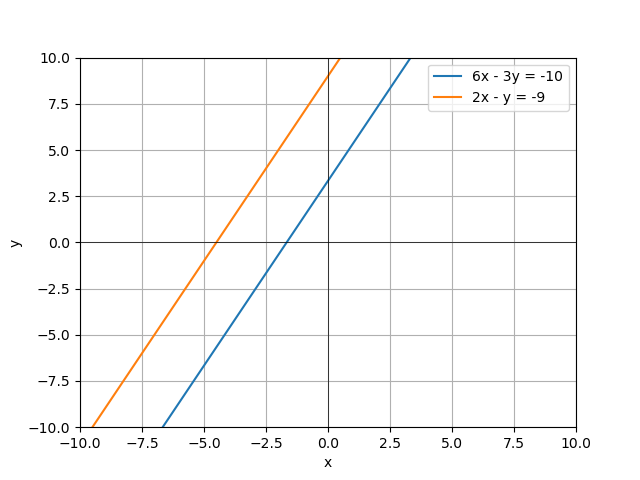
\includegraphics[width=\columnwidth]{figs/fig.png}
   \caption{Plot of the lin $6x - 3y+10$ and $2x-y+9=0$}
   \label{stemplot}
\end{figure}
\end{frame}
\subsection{Code}
\begin{frame}{Codes}
   Code: https://github.com/Balaji29-code/EE1003/tree/main/Problem-6/codes
\end{frame}





\end{document}


